\begin{frame}[t]{Alkaloiden - Klassifizierung}
\begin{quote}
  Die \enquote{echten} Alkaloide werden nach den in ihnen enthaltenen
  heterocyclischen Ringsystemen eingeteilt.
\end{quote}
  \begin{table}[htpb]
    \tiny
    %\caption{Wichtige Gruppen der Alkaloide mit Aminosäurenvorstufen}
    \begin{tabular}{llll}
      \hline
      Strukturgruppe & Alkaloid Gruppe & Vorstufe & Beispiele \\
      \hline
      \chemfig[][scale=0.5]{
        =^[:270]% 2
        -[:330]% 3
        =^[:30]% 4
        -[:90]% 5
        (
        =^[:150]% 6
        -[:210]% -> 1
        )
        -[:30]% 7
        =_[:330]% 8
        -[:270]% 9
        =_[:210]N% 10
        (
        -[:150]% -> 4
        )
      }& Chinolin & Tryptophan & Chinin \\
      \multirow{3}{*}{\chemfig[][scale=0.5]{
        -[:300.8]N% 2
        -[:279.7]% 3
        -[:233.9,1.069]% 4
        -[:31.3,0.88]% 5
        -[:65.7,0.943]% 6
        (
        -[:141.9,0.864]\phantom{N}% -> 2
        )
        -[:1,1.126]% 7
        -[:279.6,1.005]% 8
        (
        -[:30,,,1]OH% 10
        )
        -[:140.3,0.813]% 9
        (
        -[:180,1.178]% -> 3
        )
    } } &  &  & Cocain \\
        & Tropan & Ornithin& Scopolamin\\
        && & Hyoscyamin\\
        &&&\\
        &&&\\
   \multirow{4}{*}{\chemfig[][scale=0.5]{
        R=[:0]% 6
       -[:300]% 5
       =^[:0]% 4
                 (
           -[:300]% 34
                     (
            -[:0,,,1]OH% 36
                     )
           =[:240]O% 35
                 )
    -[:60,,,1]NH% 3
    -[:120,,1]% 2
                 (
           -[:180]% 1
           -[:240]% -> 6
                 )
        <[:60]% 37
                 (
           =[:120]O% 38
                 )
    -[:0,,,1]OH% 39
    } } & Betalaine & Tyrosin & Betanidin \\
        && & Indicaxanthin\\
        &&&\\
        &&&\\
        &&&\\
        &&&\\
\multirow{4}{*}{\chemfig[][scale=0.5]{
    =^[:270]% 2
     -[:330]% 3
     =^[:30]% 4
      -[:90]% 5
               (
        =^[:150]% 6
         -[:210]% -> 1
               )
      -[:18]% 7
    =_[:306]% 8
     -[:234]\chembelow{N}{H}% 9
               (
         -[:162]% -> 4
               )
    } } & Indol & Tryptophan & Harmin \\
        && & Ergolin\\
        && & Strychinin\\
        && & Reserpin
    \end{tabular}
  \end{table}

\end{frame}
\begin{frame}[t]{Alkaloide - Klassifizierung}
   \begin{table}[htpb]
    \tiny
  %  \caption{Wichtige Gruppen der Alkaloide - II}
    \begin{tabular}{llll}
      \hline
      Strukturgruppe & Alkaloid Gruppe & Vorstufe & Beispiele \\
      \hline
      \multirow{3}{*}{\chemfig[][scale=0.5]{
    =^[:270]% 2
     -[:330]% 3
     =^[:30]% 4
     -[:330]% 5
     =^[:30]N% 6
      -[:90]% 7
    =^[:150]% 8
     -[:210]% 9
               (
         -[:270]% -> 4
               )
    =^[:150]% 10
               (
         -[:210]% -> 1
               ) 
    } } & Isochinolin & Tyrosin & Morphin \\
        && & Codein\\
        && & Papaverin\\
   \chemfig[][scale=0.5]{
       =^[:180]% 2
     -[:240]% 3
    =^[:300]N% 4
           -% 5
     =^[:60]% 6
               (
         -[:120]% -> 1
               )
    }  & Pyridin & Ornithin & Nicotin \\
\multirow{4}{*}{\chemfig[][scale=0.5]{
     =_[:330]% 2
     -[:270]% 3
               (
         -[:342]N% 7
         =^[:54]% 8
         -[:126]\chemabove{N}{H}% 9
         -[:198]% -> 2
               )
    =_[:210]N% 4
     -[:150]% 5
     =_[:90]N% 6
               (
          -[:30]% -> 1
               )
    } } & Purin & Glycin & Adenin \\
        && & Guanin\\
        && & Theobromin\\
        && & Coffein
    \end{tabular}
  \end{table}

 
\end{frame}
  \begin{frame}[t]{Alkaloide - weitere Einteilung}
    \begin{quote}
      Angehörige einer dieser Alkaloidgruppen können weiter nach am genannten
      Ringsystem ankondensierten zusätzlichen Ringen bestimmten Typen zuordnen. \footnotemark  
    \end{quote}
  
  \begin{columns}[onlytextwidth,t]
    \begin{column}{0.3\textwidth}
      \begin{minipage}[c][0.9\textheight][l]{\linewidth}
       \begin{figure}
    \centering
    \textbf{Ergolin}\par\medskip
        \includegraphics[height=2cm]{data/ergot/ergolingerust}% Place your graphic here
\end{figure} 
      \end{minipage}
    \end{column}
    \begin{column}{0.3\textwidth}
   \begin{minipage}[c][0.9\textheight][l]{\linewidth}
       \begin{figure}
    \centering
    \textbf{Ergolin-Typ}\par\medskip
        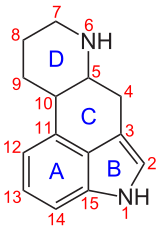
\includegraphics[height=2cm]{data/ergot/ergolinabcd}% Place your graphic here
\end{figure} 
      \end{minipage}
    \end{column}
   \begin{column}{0.3\textwidth}
      \begin{minipage}[c][0.9\textheight][l]{\linewidth}
     \begin{itemize}
       \item The base of ergot alkaloids is the tetracyclic ergoline ring
         system  
     \end{itemize}
      \end{minipage}
    \end{column}
  \end{columns}

\end{frame}

\begin{frame}[t]{Alkaloiden Typen}

  \begin{itemize}
    \item Indol Alkaloid-Typen: Strychinin, Yohimbin, $\beta$ - Carbolin,
      Physostigmin  ...
    \item Isochinolin-Typen: Morphinan-Typ (Morphin, Codein),
      Benzylisochinolin-Typ (Papaverin) (14 Typen)
    \item Tropanalkaloiden Typen:   
  \end{itemize}
  

\end{frame}

\begin{frame}[t]{Einteilung nach Vorkommen}
 
  \begin{table}[htpb]
    \centering
    %\caption{caption}
    %\label{tab:label}
    \begin{tabular}{llll}
      Familie & &Art & Alkaloide  \\
      Solanaceae & & Nicotina Rustica & Nicotin  \\
    \end{tabular}
  \end{table}
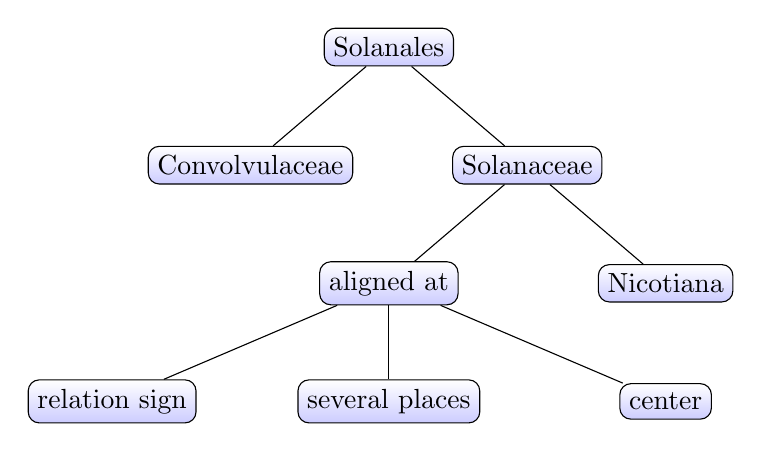
\begin{tikzpicture}[sibling distance=10em,
  every node/.style = {shape=rectangle, rounded corners,
    draw, align=center,
    top color=white, bottom color=blue!20}]]
  \node {Solanales}
    child { node {Convolvulaceae} }
    child { node {Solanaceae}
      child { node {aligned at}
        child { node {relation sign} }
        child { node {several places} }
        child { node {center} } }
      child { node {Nicotiana} } };
\end{tikzpicture}
\end{frame}
